\documentclass[tikz,border=5pt]{standalone}
\usepackage[UTF8]{ctex}
\usepackage{amsmath,amssymb}
\usetikzlibrary{arrows.meta,calc}
\definecolor{ink}{HTML}{243447}\definecolor{blue}{HTML}{2765A2}
\definecolor{green}{HTML}{3F7D5B}\definecolor{red}{HTML}{B74739}
\tikzset{body/.style={draw=ink,thick},vec/.style={draw=blue,thick,-{Latex}},
guide/.style={gray!60,dashed},dim/.style={ink,{Latex}-{Latex}},
line cap=round,line join=round}
\begin{document}
\begin{tikzpicture}
% 两个六元环、18个链碳与10个甲基碳，共40个碳；11个共轭双键。
\draw[body](0,0)--(0,-.8)--(-.6928,-1.2)--(-1.3856,-.8)
--(-1.3856,0)--(-.6928,.4)--cycle;
\draw[body](-.10,-.075)--(-.10,-.725);
\draw[body](-.6928,.4)--(-1.1128,.82);
\draw[body](-.6928,.4)--(-.2728,.82);
\draw[body](0,-.8)--(.47,-1.071);
\foreach\k in{0,...,17}{
\pgfmathsetmacro{\px}{.6*(\k+1)}
\pgfmathsetmacro{\py}{.3*mod(\k+1,2)}
\coordinate(P\k)at(\px,\py);}
\draw[body](0,0)--(P0);
\foreach\k in{0,...,16}{
\pgfmathtruncatemacro{\kp}{\k+1}
\draw[body](P\k)--(P\kp);}
\foreach\k in{0,...,8}{
\pgfmathtruncatemacro{\even}{2*\k}
\pgfmathtruncatemacro{\odd}{2*\k+1}
\draw[body]($(P\even)!.12!(P\odd)+(0,-.085)$)
--($(P\even)!.88!(P\odd)+(0,-.085)$);}
\foreach\k in{2,6}\draw[body](P\k)--++(0,.62);
\foreach\k in{11,15}\draw[body](P\k)--++(0,-.62);
\draw[body](P17)--(11.4,.3);
\draw[body](11.4,.3)--(11.4,1.1)--(12.0928,1.5)
--(12.7856,1.1)--(12.7856,.3)--(12.0928,-.1)--cycle;
\draw[body](11.50,.375)--(11.50,1.025);
\draw[body](11.4,1.1)--(10.93,1.371);
\draw[body](12.0928,-.1)--(11.6728,-.52);
\draw[body](12.0928,-.1)--(12.5128,-.52);
\node at(5.7,1.9){$\beta$-胡萝卜素：$\mathrm C_{40}\mathrm H_{56}$};
\draw[blue,line width=1.5pt](0,-2.15)--(0,-2.9)--(11.4,-2.9)--(11.4,-2.15);
\node[text=blue]at(5.7,-2.15){等效一维区间，$V=0$};
\draw[dim](0,-3.4)--(11.4,-3.4)node[midway,below]{$L$};
\node[left]at(0,-2.9){$x=0$};\node[right]at(11.4,-2.9){$x=L$};
\end{tikzpicture}
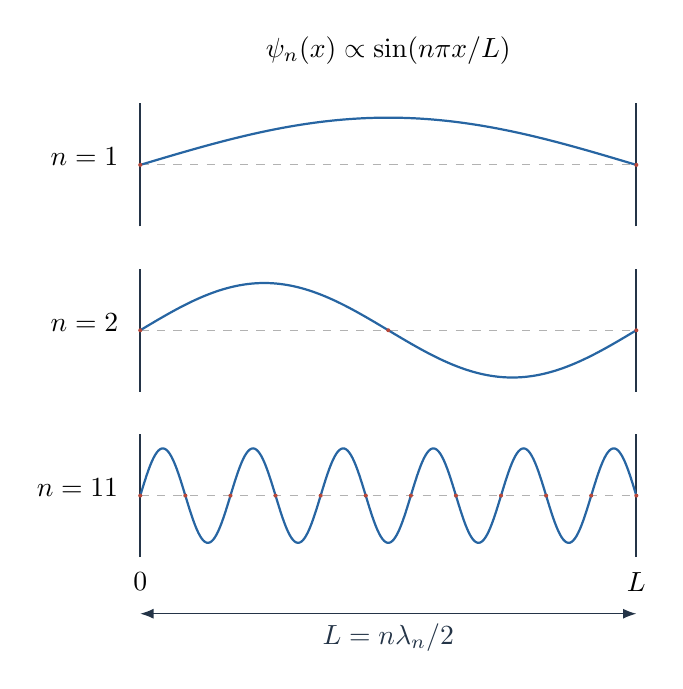
\begin{tikzpicture}[x=1.05cm,y=1cm]
\foreach\y/\n in{0/1,-2.1/2,-4.2/11}{
\begin{scope}[shift={(0,\y)}]
\draw[guide](0,0)--(6,0);
\draw[body](0,-.78)--(0,.78);
\draw[body](6,-.78)--(6,.78);
\draw[blue,thick,domain=0:6,samples=300]plot(\x,{.6*sin(\n*180*\x/6)});
\foreach\k in{0,...,\n}\fill[red]({6*\k/\n},0)circle(.025);
\node[left]at(-.15,.1){$n=\n$};
\end{scope}}
\node[above]at(3,1.15){$\psi_n(x)\propto\sin(n\pi x/L)$};
\node[below]at(0,-5.05){$0$};\node[below]at(6,-5.05){$L$};
\draw[dim](0,-5.7)--(6,-5.7)node[midway,below]{$L=n\lambda_n/2$};
\end{tikzpicture}
\begin{tikzpicture}
\draw[vec](-.4,-.45)--(-.4,5.8)node[above]{$E$};
\draw[white,line width=4pt](-.4,1.5)--(-.4,2);
\draw[ink](-.52,1.48)--(-.28,1.64);
\draw[ink](-.52,1.84)--(-.28,2.0);
\foreach\y/\n/\energy in{0/1/1,3/10/100,3.945/11/121,4.98/12/144}{
\draw[body](0,\y)--(3.3,\y)node[right]{$n=\n$};
\node[left]at(-.5,\y){$\energy E_1$};
\ifnum\n<12
\draw[blue,thick,-{Latex}](1,\y-.18)--(1,\y+.25);
\draw[green,thick,-{Latex}](1.3,\y+.25)--(1.3,\y-.18);
\fi}
\node[align=center]at(1.7,1.65){省略$n=2,\ldots,9$\\每级两电子};
\draw[red,line width=1.4pt,-{Latex}](2.6,3.945)--(2.6,4.98)
node[midway,left]{$\Delta E=23E_1$};
\node[text=red]at(1.7,5.45){最低空能级};
\node at(1.6,-.95){$22$电子填满$n=1$至$11$};
\end{tikzpicture}
\end{document}
